\chapter{Results With Data}
\label{observedresults}
\label{results}

The chapter presents the single top quark production cross section measured in nearly 1 fb$^{-1}$ of Tevatron RunII data. The cross section and the observed resolution is presented in Section~\ref{measured}. To measure the expected and observed significance psuedo-datasets with no signal contribution are created and the fraction of datasets with a measured cross section above the observed cross section is calculated. This value is the probability of a background-only fluctuation and can be converted to a Gaussian equivalent signal significance. This result is presented in Section~\ref{significance}.


%---------------------------------------------------------------------
\section{Measured Cross Section}
\label{measured}

Figure~\ref{meas-post-1d} shows the observed $tb$+$tqb$ posterior
without and with systematic uncertainties for all channels combined.

\begin{figure}[!h!tbp]
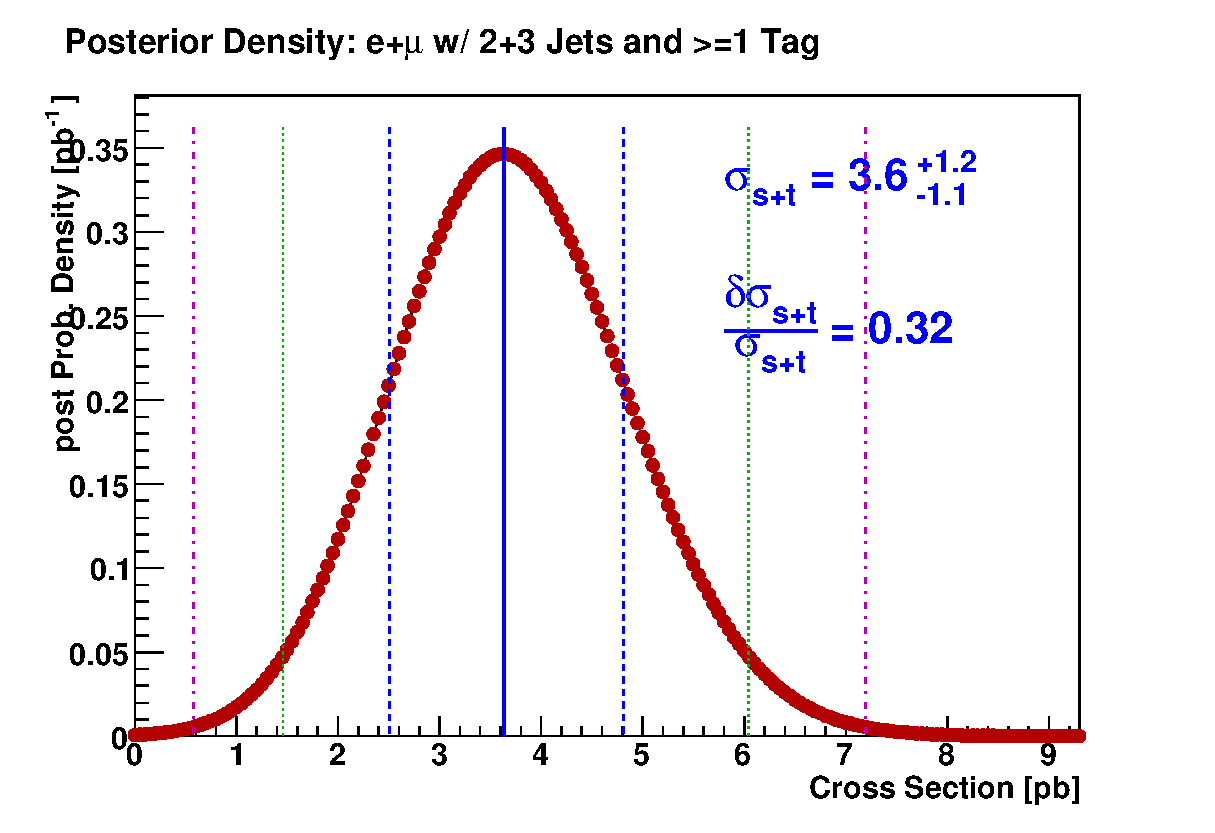
\includegraphics[width=0.49\textwidth]{eps/MatrixElement/posterior/nosys/limit_TBTQ_LeptonsCombined_JetsCombined_TagsCombined.eps}
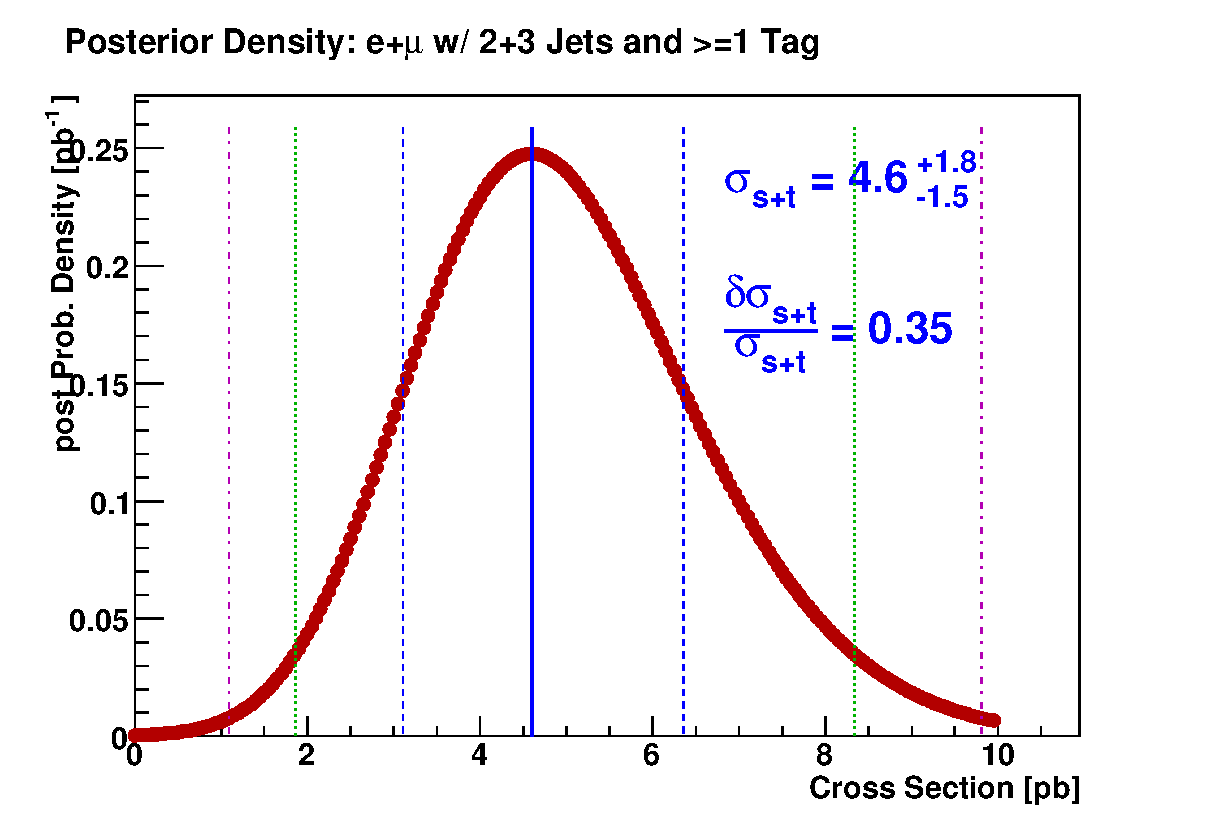
\includegraphics[width=0.49\textwidth]{eps/MatrixElement/posterior/sys/limit_TBTQ_LeptonsCombined_JetsCombined_TagsCombined.eps}
\vspace{-0.1in}
\caption{Measured 1D posterior plots for the combined
$e$+$\mu$ $\geq$~1 $B$-tag channel with statistical uncertainties only
(left plot) and with systematic uncertainties as well (right plot).}
\label{meas-post-1d}
\end{figure}

Table~\ref{tab:measxsecs} shows the measured cross sections from various combinations of analysis channels.  The averaged relative uncertainties on the measured cross sections are shown in Table~\ref{meas-errors}.

\begin{table}[!h!tbp]
\begin{center}
\caption{Measured $tb$+$tqb$ cross sections, without and
with systematic uncertainties, for many combinations of the analysis
channels. The final result of this analysis is shown in the lower
right hand corner in bold type.}
\label{tab:measxsecs}
\begin{tabular}{l|cc|cc|cc|c}
%  \multicolumn{8}{c}{\hspace{0.5in}\underline{Measured $tb$+$tqb$ Cross Section}}\vspace{0.1in}\\
& \multicolumn{2}{c|}{1,2tags + 2,3jets}& \multicolumn{2}{c|}{$e$,$\mu$ + 2,3jets}
& \multicolumn{2}{c|}{$e$,$\mu$ + 1,2tags}& All \\
                 &  $e$-chan & $\mu$-chan& 1 tag & 2 tags& 2 jets& 3 jets&channels\\
\hline
Statistics only  &  $3.0^{+1.5}_{-1.4}$  & $4.5^{+1.8}_{-1.7}$ & $2.8^{+1.2}_{-1.2}$ & $7.9^{+3.3}_{-3.0}$ & $3.5^{+1.4}_{-1.3}$ & $3.9^{+2.3}_{-2.2}$ & $3.6^{+1.2}_{-1.1}$     \\
With systematics &  $3.1^{+2.2}_{-1.8}$  & $7.4^{+3.0}_{-2.5}$ & $4.5^{+2.0}_{-1.7}$ & $6.8^{+4.7}_{-3.8}$ & $4.7^{+2.0}_{-1.7}$ & $4.9^{+3.7}_{-3.1}$ & $\mathbf{4.6^{+1.8}_{-1.5}}$     \\
\end{tabular}
\vspace{-0.1in}
\end{center}
\end{table}

\begin{table}[!h!tbp]
\begin{center}
\caption{Relative uncertainties on the measured
$tb$+$tqb$ cross section, without and with systematic uncertainties,
for many combinations of the analysis channels. The best value from
all channels combined, with systematics, is shown in bold type.}
\label{meas-errors}
\begin{tabular}{l|cc|cc|cc|c}
%  \multicolumn{8}{c}{\hspace{0.5in}\underline{Relative Uncertainties on the Measured $tb$+$tqb$ Cross Section}}\vspace{0.1in}\\
& \multicolumn{2}{c|}{1,2tags + 2,3jets}& \multicolumn{2}{c|}{$e$,$\mu$ + 2,3jets}
& \multicolumn{2}{c|}{$e$,$\mu$ + 1,2tags}& All \\
                 &  $e$-chan & $\mu$-chan& 1 tag & 2 tags& 2 jets& 3 jets&channels\\
\hline
Statistics only  &  $50\%$  & $39\%$ & $44\%$ & $40\%$ &  $37\%$  & $57\%$ & $32\%$     \\
With systematics &  $64\%$  & $38\%$ & $41\%$ & $62\%$ &  $39\%$  & $70\%$ & $\mathbf{35\%}$     \\
\end{tabular}
\vspace{-0.1in}
\end{center}
\end{table}

The combined result with full systematics is
$$
\sigma\left({\ppbar}{\rargap}tb+tqb+X\right)
= 4.6 ^{+1.8}_{-1.5}~{\rm pb}.
$$

\noindent A breakdown of the uncertainties on the $tb$+$tqb$ cross section measurement is given in Table~\ref{tab:syst}. The systematic uncertainties were calculated using an ensemble containing 200 datasets generated with an input single top cross section of 4.6~pb. The cross section of each dataset was measured and the average posterior width (average of upper and lower 1$\sigma$ uncertainties) was calculated over all datasets for each source of systematic uncertainty independently. The systematic uncertainty for each source was estimated by subtracting in quadrature from the average posterior width obtained with a particular source of systematic, the average posterior width without systematic uncertainties. The total expected systematic uncertainty is estimated by adding in quadrature all the individual expected systematic uncertainties.  The statistical uncertainty of the measurement is estimated by subtracting in quadrature the total expected systematic uncertainty from the actual total uncertainty.

\vspace{0.1in}
\begin{table}[!h!tbp]
\begin{center}
\caption{Contribution of each systematic uncertainty to the
total systematic uncertainty on the $tb$+$tqb$ cross section.}
\label{tab:syst}
\begin{tabular}{lr@{ pb~~}}
%\multicolumn{2}{c}
%{Contributions to the Cross Section Uncertainty}\vspace{0.05in}\\
\hline
\multicolumn{2}{l}{Systematics components} \\
~~Luminosity               & 0.69	\\ 
~~{\ttbar} cross section   & 0.74	\\ 
~~Matrix method            & 0.84	\\
~~Trigger                  & 0.48	\\ 
~~Primary vertex           & 0.31	\\
~~Lepton ID                & 0.50	\\
~~Jet ID                   & 0.18	\\
~~Jet fragmentation        & 0.63	\\
~~Jet energy scale         & 0.57	\\
~~Tag-rate functions       & 0.60	\\
\hline                     
Combined systematics       & +1.34~~$-1.02$ \\
Statistics                 & +1.19~~$-1.13$ \\
\hline
Total uncertainty          & +1.79~~$-1.50$ \\
\end{tabular}
\vspace{-0.1in}
\end{center}
\end{table}


Figure~\ref{xsec-summary} shows the cross sections measured for
combined the $tb$+$tqb$ production in each independent analysis channel,
and the combined result.

\begin{figure}[!h!tbp]
\begin{center}
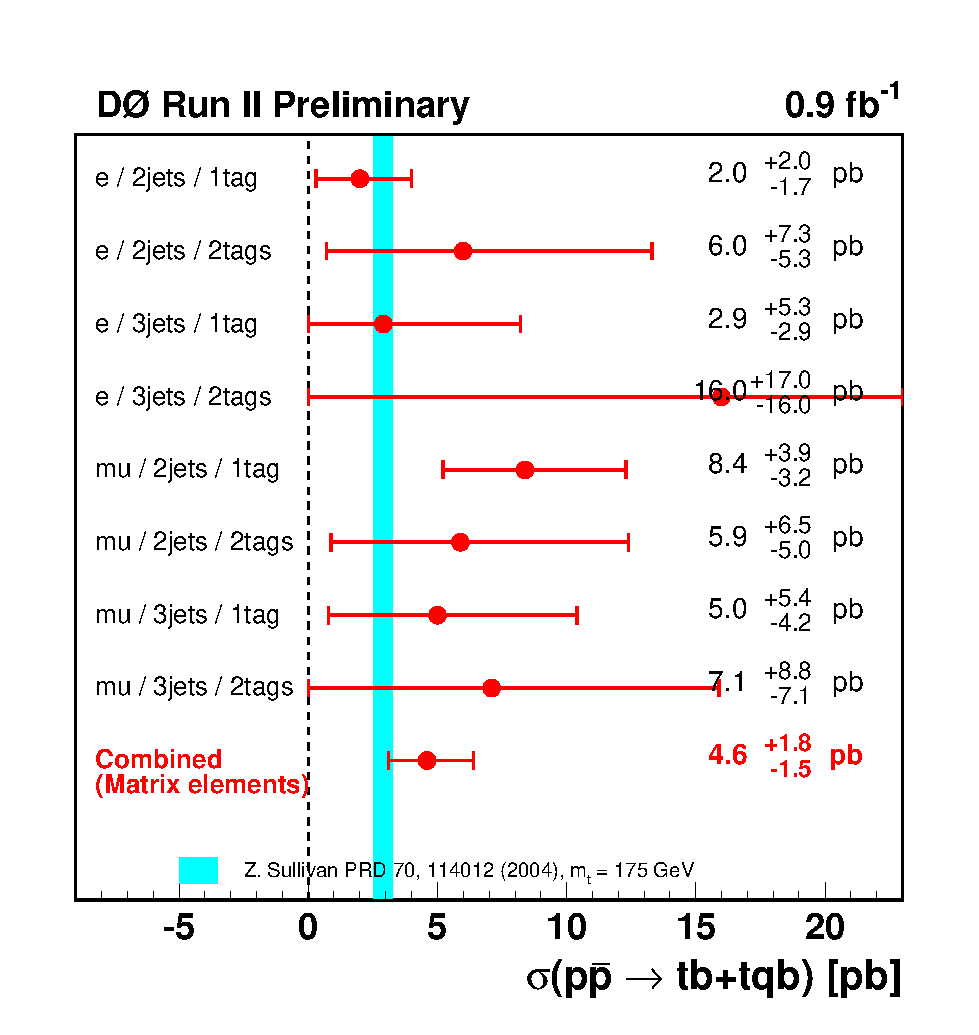
\includegraphics[width=1.00\textwidth]
{eps/MatrixElement/sintop_xsec_summary.eps}
\caption{Summary plot of the measured single top quark cross
sections showing the individual measurements and their combination.}
\label{xsec-summary}
\end{center}
\end{figure}


\section{Signal Significance and Standard Model Compatibility}
\label{significance}

The measured significance is defined as the fraction ensembles generated with zero input cross section that result in a measured cross section above the observed cross section of 4.6 pb. This quantity, known as the $p$-value, represents the probability that the background alone could fluctuate to mimic the single top quark signal. For the case of Standard Model single top the expected $p$-value is 3.7$\%$, which is equivalent to a 1.8$\sigma$ Gaussian significance of a deviation from a background fluctuation. The measured $p$-value of $0.21\%$ is equivalent to a $2.9\sigma$ significance indicating evidence for single top quark production in the dataset.


\begin{figure}[!h!tbp]
\begin{center}
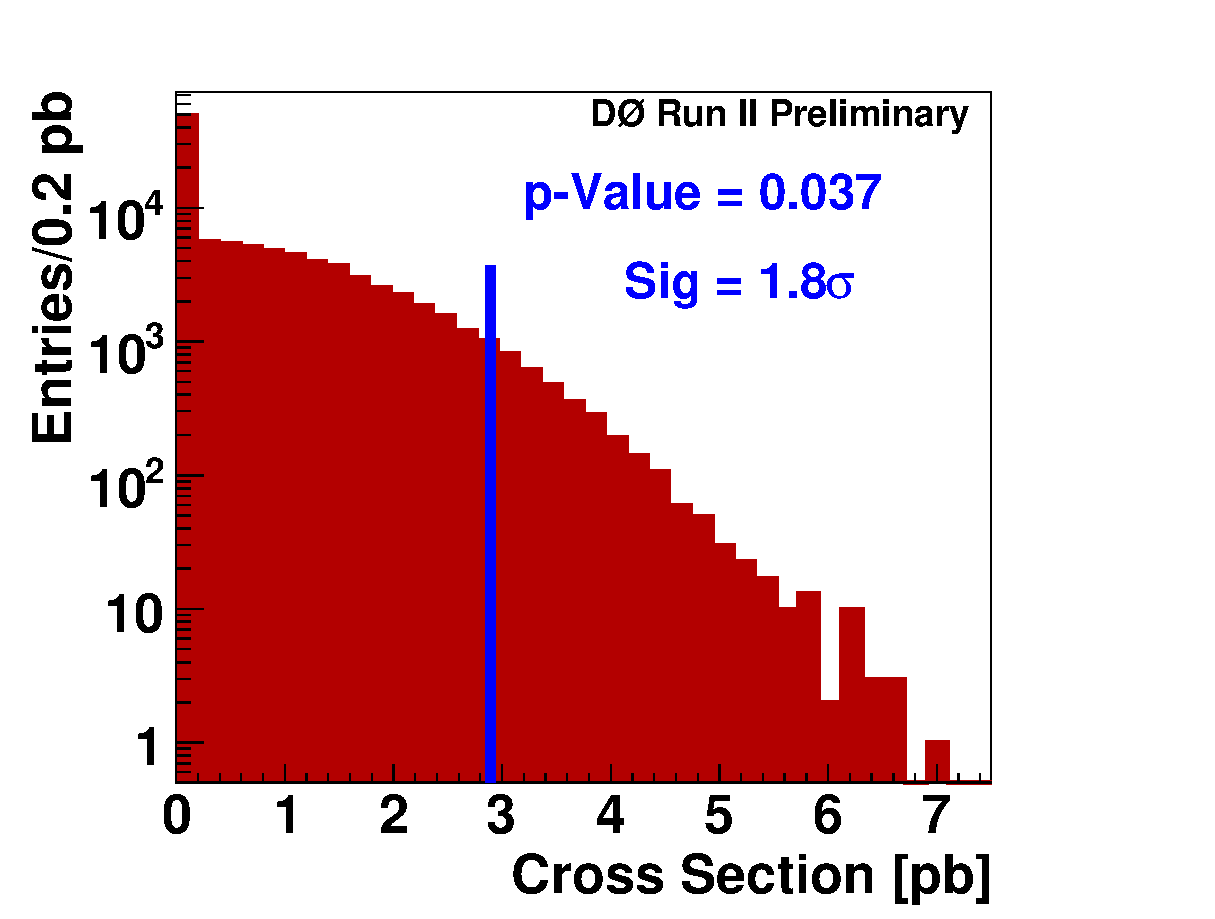
\includegraphics[width=0.48\textwidth]
{eps/Limits/ZeroSignalEnsemple_Expected.eps}
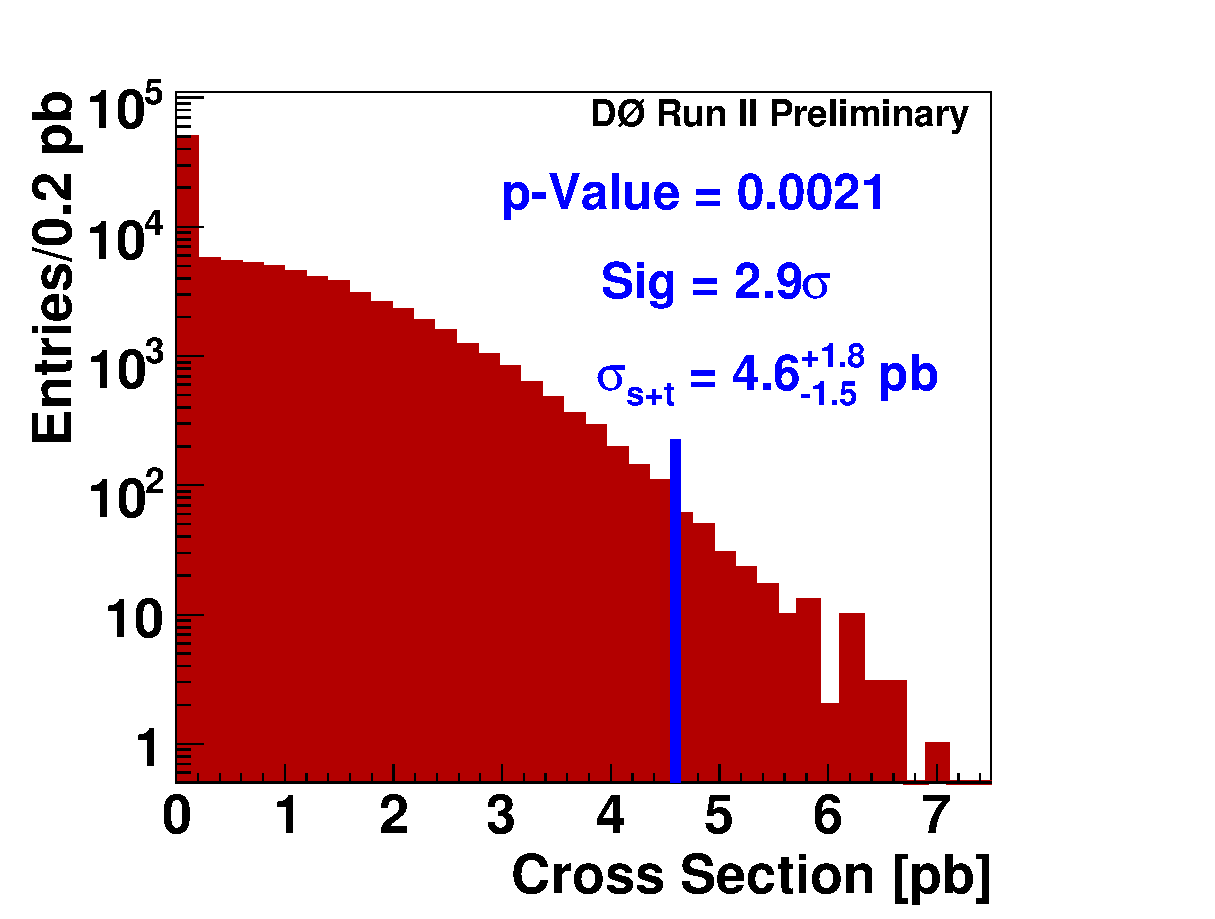
\includegraphics[width=0.48\textwidth]
{eps/Limits/ZeroSignalEnsemple_Observed.eps}
\caption{Distribution of expected (left) and measured (right) cross sections from a zero-signal
ensemble with full systematics included. The probability that the background alone could have a measured cross section above 4.6 pb or above is 0.21$\%$ leading to a Gaussian equivalent signal significance of 2.9$\sigma$.}
\label{pValue}
\end{center}
\end{figure}

The probability of a Standard Model signal to have a measured cross section above $4.6$~pb can be estimated using the Standard Model ensemble dataset (i.e. $\sigma_{s+t}=2.9$~pb). Fig.~\ref{probsm} shows the measured cross section for 2,000 Standard Model pseudo-datasets. From this histogram there is a 20.5\% probability that a Standard Model signal could be measured at or above 4.6 pb.

\begin{figure}[!h!tbp]
\begin{center}
\includegraphics[width=1.0\textwidth]
{eps/Limits/prob_sm.eps}
\caption{Distribution of measured cross sections from a Standard Model
ensemble with full systematics included. The probability that a Standard Model signal could have a measured cross section of 4.6 pb or above is 20.5$\%$.}
\label{probsm}
\end{center}
\end{figure}

